% This file is isea.tex.  It contains the formatting instructions for and acts as a template for submissions to ISEA 2015.  It is based on the ICCC  formats and instructions.  It uses the files isea.sty, isea.bst and isea.bib, the first two of which also borrow from AAAI IJCAI formats and instructions.
% Modified from ICCC.tex by B. Bogart

\documentclass[letterpaper]{article}
\usepackage{isea}
\usepackage[pdftex]{graphicx}
\usepackage{times}
\usepackage{helvet}
\usepackage{courier}
\usepackage[numbers]{natbib}
\pdfinfo{
/Title (ISEA2015 Formatting Instructions for Authors)
/Author (ISEA 2015)}
% The file isea.sty is the style file for ISEA 2015 proceedings.
%
\title{ISEA2015 Formatting Instructions for Authors}
\author{1\textsuperscript{st} Author Name, 2\textsuperscript{nd} Author Name,  \ldots, n\textsuperscript{th} Author Name\\
Affiliation(s)\\
Location, Country\\
Contact Emails\\
\newline
\newline
}
\setcounter{secnumdepth}{0}

\begin{document} 
\maketitle
\begin{abstract}
The Proceedings of the International Symposium on Electronic
Art will be compiled from electronic manuscripts submitted by
the authors. This paper provides brief style instructions that will
facilitate high-quality, consistent, proceedings. The title
``Abstract'' should be 10 point, bold type, centered at the
beginning of the left column. The body of the abstract
summarizing the thesis and conclusion of the paper in no more
than 200 words should be 9 point, justified, regular type.
\end{abstract}

\section{Keywords}

The title ``Keywords'' should be 10 point, bold type, centered at the beginning of the left column. Using 9 point, justified, regular type, write up to ten keywords that highlight the main areas of your essay’s content. 

\section{Introduction}

Your essay’s heading should be 12 point, bold style, centered. Your body text should be 10 point, justified, single space. The first sentence after the heading begins without a paragraph indent like this paragraph.

The second, and subsequent paragraphs are indented 10 points. Do  not  leave  double-space  between   words  or  paragraphs. This sample shows a 10-point Times New Roman text. Times New  Roman  is  the font to be used throughout the essay.

The ISEA2015 submission must be PDF (Portable Document Format) files formatted for 8-1/2'' x 11'' paper.

\subsection{Word Processing Software}

As detailed below, ISEA has prepared and made available a Microsoft Word template and an Open Office template for use in formatting your paper. If you are using some other word processing software, please follow the format instructions given below and ensure that your final paper looks as much like this sample as possible.

\subsection{Length of Papers}

A variety of paper lengths will be accepted under different categories. Please note that submission lengths must be all inclusive (including references, biographies and acknowledgements).
\begin{itemize}
\item Long paper submissions can be up to 8 pages in the ISEA2015 template format.
\item Art and Research short paper submissions can be up to 4 pages in the ISEA2015 template format.
\item Extended abstract submissions can be up to 2 pages in the ISEA2015 template format.
\item Round tables and square panel submissions can be up to 2 pages in the ISEA2015 template format.
\item Institutional presentation submissions can be up to 2 pages in the ISEA2015 template format.
\end{itemize}

\section{Style and Format}
Templates that implement these instructions can be retrieved electronically at {\small \tt http://isea2015.org}

\subsection{Layout}

Print manuscripts two columns to a page, in the manner in which these instructions are printed. The exact dimensions for pages are:
\begin{itemize}
\item left and right margins: 0.75''
\item column width: 3.31''
\item gap between columns: 0.38''
\item top margin—first page: 1.25''
\item top margin—other pages: 0.75''
\item bottom margin: 1.25''
\end{itemize}

\subsection{Format of Electronic Manuscript}

For the production of the electronic manuscript, you must use {\em Adobe's Portable Document Format} (PDF). Additionally, you must specify the American {\em letter} format (corresponding to 8-1/2'' x 11'') when formatting the paper.

\subsection{Blind Review}

All papers will be reviewed in a single blind manner.  You are at liberty to include your affiliation and cite your papers in a natural manner, and you are also at liberty to anonymize the text if you so desire, in which case, keeping your identity secret is your responsibility.

\subsection{Title and Author Information}

Center the title on the entire width of the page in a 16-point bold font. Below it, center the author name(s) in a 12-point bold font, and then center the address(es) in a 9-point regular font. Credit to a sponsoring agency can appear in the Acknowledgment Section described below.

\begin{figure}[h]
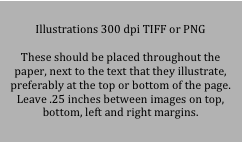
\includegraphics[width=3.31in]{figure.png}
\caption{This is an example of figure caption. Note that all figures, and tables are to be referenced in the text. \copyright Respect Copyright.}
\end{figure}

\subsection{Abstract}

The title ``Abstract'' should be 10 point, bold type, centered at the beginning of the left column. The body of the abstract summarizing the thesis and conclusion of the paper in no more than 200 words should be 9 point, justified, regular type.

\subsection{Text}

The main body of the text immediately follows the abstract. Use 10-point type in {\em Times New Roman} font.

Indent when starting a new paragraph, except after major headings. 

\subsection{Headings and Sections}

When necessary, headings should be used to separate major sections of your paper. (These instructions use many headings to demonstrate their appearance; your paper should have fewer headings.

\subsubsection{Section Headings}

Print section headings centered, in 12-point bold type in the style shown in these instructions. Your body text should be 10 point, justified, single space. Do not number sections.

\subsubsection{Subsection Headings}

Print subsection headings left justified, in 11-point bold type and mixed case (nouns, pronouns, and verbs are capitalized). They should be flush left. Your text should be 10 point, justified, single space. Do not number subsections.

\subsubsection{Subsubsection Headings}

Print subsubsection headings inline in 10-point bold type. Do not number subsubsections.

\subsubsection{Special Sections}

You may include an unnumbered acknowledgments section, including acknowledgments of help from colleagues, financial support, and permission to publish.

The references section is headed ``References,'' printed in the same style as a section heading. A sample list of references is given at the end of these instructions.  Note the various examples for books, proceedings, multiple authors, etc. 

\subsection{Footnotes}

If footnotes are necessary, place them at the bottom of the page in 9-point font. Refer to them with superscript numbers.\footnote{This is how your footnotes should appear.} Separate them from the text by a short horizontal line. 

\subsection{Itemized Lists}

Itemized lists shall use the en-dash as item. Let’s take the case of URL, automatic links and punctuation as an example:
Turn off the automatic linking feature for URLs in Word.

Quotations: For direct quotations remember to use ``double inverted commas.'' Quotations must be carefully transcribed and accurate. 

Periods and commas go inside quotation marks. This applies to ``double inverted commas,'' as well as single `inverted commas,' and to the use of a full stop as in the ``following example.'' 

Parenthesis: When an entire sentence is enclosed in parentheses, the punctuation mark belongs inside the closing parenthesis as in this example: applying this may be difficult at times. (We think it is important.)

\begin{itemize}
\item The punctuation mark belongs outside the closing parenthesis if the brackets are within the sentence as in this example: applying this may be difficult at times, but good results are guaranteed (and this is important).
\item Use en dashes with spaces -- like this -- to set off phrases. En dashes are moreover placed between digits to indicate a range (1--10 October; pp. 25--30). You can type an en dash with ALT + 0150 (in the numeric keypad) in Windows, or OPTION + HYPHEN in Mac.
\end{itemize}

\subsection{Quotations and Extracts}
Indent long quotations and extracts by 10 points at left margins.

\section{Acknowledgments}
The preparation of these instructions and the \LaTeX{} and Word files was facilitated by borrowing from similar documents used for ICCC proceedings.

\begin{figure*}

\includegraphics[width=\textwidth]{two-column-figure.png}
\caption{Example of a double-column figure with caption. \copyright Respect Copyright.}
\end{figure*}

\section{Bibliography}
The title ``Bibliography'' should be 12 point, bold style, centered. Using 9 point, regular type, list your bibliography in alphabetical order by family name, after the references. The difference between a reference list and a bibliography is that in your references, you list all the sources you directly referred to in the body of your writing in numerical order, whereas a bibliography includes an alphabetical listing of all those authors and sources that you have consulted while writing your essay. Use the same format as for the references otherwise. Those using Latex will follow the usual cite command format \cite{boden92}.

\section{Author(s) Biography(ies)}
The title ``Author(s) Biography(ies)'' should be 12 point, bold style, centered. Using 9 point, regular type, biographies should be no longer than 150-word count.

\section{Questions?}

For technical questions about Microsoft Word formatting please seek online tutorials. For other questions about your manuscript please contact: {\tt ISEA2015-info@sfu.ca}


\bibliographystyle{isea}
\bibliography{isea}


\end{document}
